\documentclass[a4paper,man,12pt,apacite]{apa6} % man => jou
\usepackage[english]{babel}
\usepackage[utf8]{inputenc}
\usepackage{mathtools}
\usepackage{url}

\begin{document}

\title{Random Forests Destructured: Introduction, Overview, Possibilities}
\shorttitle{Random Forests Destructured}
\author{Tobias Ammann}
\keywords{ensemble methods, introduction, random forests}
\affiliation{Literature Study at the Workgroup for Psychological Methods,\\Evaluation and Statistics, Department of Psychology.\\Supervised by Prof. Dr. Carolin Strobl}

\abstract{This report a rather new machine learning algorithm called
"Random Forests", its qualities, use, problems, and a small number of
improvements that have been tried.
Random forests are getting a lot of attention outside of psychology,
and it would be nice to encourage their application within psychology too.
However, it is important to keep in mind that random forests are
relatively unstudied. This hasn't hindered a number of people to suggest
improvements. This paper tries to give the reader a practical
understanding of the method, which hopefully leads to a better
application random forests.}

\keywords{ensemble methods, introduction, random forests}

\maketitle

\tableofcontents

\section{Introduction}

\subsection{Motivation}
Psychology has become a science, thus psychological research has to follow
the \emph{scientific method}, according to which positive proof is an
impossibility unless we have complete knowledge, and could eliminate all
alternative theories.
However, we won't ever have complete knowledge, therefore scientific isn't
about proofs, but probabilities.
Research works under the assumption that if we disprove just enough
alternative theories, we can eventually tell which theory is probably
true.
So, the scientific method really is nothing but the use of countless
attempts to disprove alternative theories, until only a single such theory
remains.

Since there is an unweildly number of theories to disprove, and every
researcher likes to see the result of his work during his lifetime, a
more speedy method is usually employed, although this comes with a caveat.
The speedier method has the researcher pit his favored theory against
the null hypothesis, a fancy word for chance.
This is way more efficient than comparing the thousands of
theories that researchers have come up with, and continue to come up with.
The caveat, commonly called confirmation bias, is that the result only
has significance in the experimental set-up being tested.
In the greater scale of things, i.e. reality, the results might well be
completely bogus.
Nonetheless, most of the subjects being studied are sufficiently constant
or change predictably enough to allow researchers to generalize from the
results of an experiment to the world at large, and likely remain correct.
This likelihood depends on the size of the effects measured in the
experiment, the number of experimental subjects, and on the properties of the
statistical methods involved.
In psychological research, where large effects are rare and
experiments usually study only a handful of psychology students, it is
vital to use good statistical methods, because that is the only parameter
remaining for the researcher to tweak in his favour.

Recently, researchers in psychology began to turn to a new breed of
statistical methods, in hope of ever better results. This new breed of
statistical methods is called \emph{machine learning}.

In this paper, I aim to introduce the reader to \emph{random forests},
which are just one family of algorithms.
I intend to do this in a way that gives every reader a chance to understand
this method without prior knowledge. I also intend to present the reader
with some context around random forests, in hope that they will benefit
from a more big-picture view.

In the next sections I introduce the reader to machine learning,
the differences between the traditional statistical and this new
machine learning approach, random forests in particular, and finally delve
into some improvements to random forests that have been suggested in the
literature.

\subsection{Machine Learning}
In order to understand random forests, it might be useful to set
the stage by briefly discussing machine learning in general.
Machine Learning is both a part of predictive statistics and the
artificial intelligence branch of computer science.

\emph{Predictive statistics} is the sub-field of statistics that is
concerned with making predictions based on past observations.
It's probably most widely known method is \emph{linear regression}
\cite{wpLR} that associates two variables \(y\) and \(x\) in such a way
that they describe a straight line: \(y = \alpha * x + \beta \).
Predictive statistics is widely used in psychology because it
allows the researcher to look at the unobservable by making
assumptions of the form \(reaction = mind * stimulus + variation\).
This is the standard approach in personality questionaires.

\emph{Artificial intelligence} is a field commonly associated with the
computer sciences, where it began with the advent of higher-order
programming languages based on mathematical foundations around the \emph{1960s} \cite{wpHOPL}.
Its aim is to give computers human-like capabilites, so that they can assist
us by combining intelligence, with flawless logic and super-human knowledge.
It includes things like \emph{logic programming} \cite{wpLP},
\emph{expert systems} \cite{wpES}, \emph{databases} \cite{wpDB} and
\emph{neural networks} \cite{wpNN}, that all represent some form of
storing and querying knowledge.
Unfortunately, early computers back then didn't have the speed and memory
required to push the envelope far enough, and the field was deemed dead.
Only the rather recent coexistance of powerful computers and massive amounts
of stored data, sometimes called \emph{big data}, revived artificial
intelligence as an important field of research.

\emph{Machine learning} is that part of artificial intelligence that
is concerned with the computer's learning of facts about the world.
These facts can then be stored and subsequently queried later on.
As such machine learning is concerned with making statements based
on past observations, and, is therefore, close to predictive statistics
\cite{wpML}.

\subsection{The Machine Learning Life Cycle}
This section discusses the difference between machine learning and traditional
statistical methods. Terminology.
The following section heavily relies on information found in Wikipedia, as
well as what I learned in statistics lectures in the past years.
A good introductory article is \cite{wpML}.

Traditionally, the statistical methods used in psychology
take a model of how the world works, and a set of data, and return one of
two things.
They either return a probability of how likely an improvement in prediction
can be observed at random, or how likely a difference in measurement can be
observed at random.

\emph{Regression methods} try to derive the values of
one variable from the other variables in the dataset using a formula the
researcher specifies.
They then compare the actual values and the prediction my the model with
different inputs, and calculate how probable an improvement in this
comparison is to show up due to random variations \cite{wpRA}.

\emph{Analysis of variance methods} partition the dataset
according to all but one variable. They then calculate the probability with
which the variation in the one variable among the groups could be due to
random variations in the dataset \cite{wpAOV}.

The probabilities the methods output are what statisticians call the
significance. Statisticians usually define a target significance level,
e.g. 5\%, and compare it to the output of their statistical calculations.
If the calculated probability is less than the targeted significance level the
measured effects are said to he significant at the chosen significance level.
For example, a result that is significant at 5\%, we know that it is less
likely to show up at random than in 5\% of all experiments.

The most striking difference between traditional statistical methods and
machine learning methods is that the researcher can't specify his model of
how the world works, other than through the selection of a machine learning
algorithm.
Because of this, machine learning algorithms are sometimes described as
\emph{black boxes}, meaning that the user can only see what's going into the
algorithm, and what is coming out.
This is unlike the statistical methods, where the researcher supplies a
formula, because in machine learning, algorithms derive the model on their own.
This is what the learning in machine learning means.
The second difference is what the algorithms return.
Since machine learning algorithms represent the model, what they output is
not a percentage, i.e. significance, but the model itself.
In short, machine learning provides the researcher with a generic model
that adapts to the world.
The prediction of such a model can then be calculated for data for which
the values of the output variable are known, but that hasn't
been included in the learning phase, to calculate the significance.
The problem with this flexibility is, that one cannot really tell what the
model looks like, that is, the model is not in a human-readable form.
As will be pointed out later, decision trees, the underlying mechanism in
random forests, are quite easily understandable, but random forests
consist of dozens to thousands of such trees, so that a human can hardly
tell what they mean.
Therefore, it is very important to find ways to condense this complexity
into something that can be more easily interpreted.
The variable importance measure of random forests, which will be introduced
later, is one such way.

\subsection{Classification}
The \emph{classification problem} is the problem of classifying new data based
on a set of example data, but without the explicit set of rules that guided the
classification of the example data.
Unlike in \emph{regression}, the result here is one of many given classes
and not a numeric value.
One might describe classification as regression with discreet output values.
Output variables are commonly called \emph{classes}, while input variables
are commonly called \emph{features} independent of the type of problem.

\subsection{Regression}
A short discussion of regression, the why and how, and the difference
between classical regression and regression in machine learning.
Terminology. Classification with continuous classes.

\subsection{Randomness}
Many machine learning algorithms consume random numbers in different places.
While computer generated random numbers are not truly random, they still
cause the outcome of the algorithm to change slightly between different
executions, due to the fact that they are customarily initialized with
the current time at the start of the program.
These changes might unnerve a novice, but don't change the outcome of the
algorithm significantly.
Still, for publication purposes it can make sense to set and publish the
random number generator's \emph{seed}, i.e. the value the generator is being
initialized with.
However, doing so during the experiment
is a serious mistake.
Indeed, it is good practice to run the analysis multiple times to ensure
that these random variations don't change the outcome.

\section{Random Forests}

\subsection{Ensemble Methods}
A short introduction to ensembles and their properties. Terminology.
Weak and strong learners. \cite{dietterich2000experimental}
\cite{bauer1999empirical}

\subsubsection{Bootstrapping}
Sampling the data.

\subsubsection{Random Subspaces}
Sampling the variables.

\subsubsection{Boosting}
Weighing the sample.

\subsection{Trees and forests}
The \emph{trees} computer scientists refer to are artificial constructs that
branch out starting from a single point, called \emph{root node}.
A common \emph{fan-out factor} is two, meaning that every node in the tree
as two branches connecting it to two other nodes.
These two nodes are called \emph{child nodes}.
Nodes without child nodes of their own are called \emph{leaf nodes}.
Keeping with the reference to nature, the word \emph{forest} denotes a
collection of trees \cite{wpTREE}.

\subsubsection{Decision Trees}
A \emph{decision tree} is a tree structure that sketches a decision process:
every node stands for a criterion, and leaf nodes denote outcomes.
To use a decision tree, one starts at the root node, and follows the path
along those nodes whose criteria are met, until a leaf node is reached, i.e.
the outcome of the decision process.

A decision tree from an economics context as an example \cite{wpDT}.
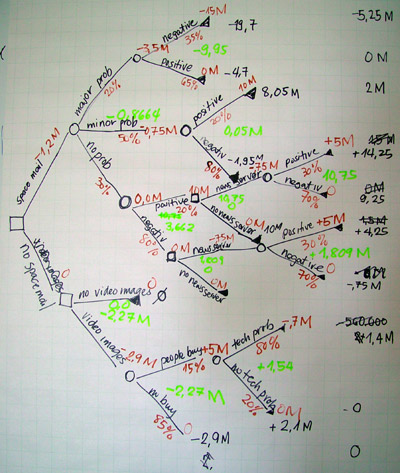
\includegraphics[width=0.4\textwidth]{WikipediaMDT.jpg}
\\

The advantage of decision trees is, that they can be constructed by an
algorithm, but still provide meaningful information to a human reader.
The reader can easily see which criteria lead to which decision.

\subsubsection{Random Forests}
Random forests were invented by Leo Breiman.
The following description is based on his original publication in the
journal \emph{Machine Learning} in 2001 \cite{breiman2001random}.

\emph{Learning and Predicting}

\emph{Variable Importance}

\subsection{In Search of the Super-Tree}
The fact that the random forest method is still being studied, that its
optimal parameter settings are still being debated, and that its results
are not always better than other methods, led to the development of
variants.
Every variant tries to address a specific problem, tries to increase the
learning efficiency or tries to better prevent overfitting.

\subsubsection{Alternative: Dynamic Random Forests}
Boosting random forests.

\subsubsection{Alternative: PERT}
Random variables and random splits.

\subsubsection{Alternative: Rotation Forest}
Massaging features before growing trees.

\subsubsection{Alternative: Fuzzy Random Forests}

\section{Method}

\subsection{Selection of Papers}
I started my research on \emph{random forests} by reading the
introductory paper suggested by my supervisor titled
\emph{An introduction to recursive partitioning: Rationale, application
and characteristics of classification and regression trees, bagging and
random forests} \cite{strobl2009introduction}.
I then searched the research databases \emph{PsychARTICLES} and
\emph{PsychINFO} querying for \emph{random forest} and limiting my results
to the last two years.
I only considered papers that focus on \emph{random forests} and
dismissed every paper where \emph{random forests} are merely used as a
research method.
I also used \emph{Google Scholar} to look for more technical
publications outside the field of psychology.
I searched for combinations of \emph{random forest}, \emph{comparison},
\emph{analysis}, and \emph{ensemble}.
I also included keywords seen in interesting titles, like \emph{fuzzy},
\emph{perfect}, \emph{full}, \emph{balanced}, \emph{extremely}, and
\emph{rotation}.
I also queried for some of the referenced publications while I read the
found material, but only included \cite{strobl2008conditional}, because
it was referenced multiple times, and co-authored by this paper's
supervisor.

The final criteria for inclusion were the online availability of a freely
downloadable PDF-file, which thanks to \emph{Google Scholar} often turned
out to be no problem at all, and my decision on the topic of
this report.

A lot of the information in the fields of computer science, artificial
intelligence, machine learning, databases, and especially programming
I acquired through different means in the last ten years.
As I couldn't remember the original sources, I can only include the pages
on Wikipedia, which I used to refresh my memories.

\subsection{Aim and Structure of the Paper}
Possible options for this topic were the presentation of
exemplary uses of random
forests, the discussion of strengths and weaknesses, and any of the more
specialized variants.
During my research I had the impression, that there were serious
differences in the understanding of random forests among researchers,
and even among designers of improved variants.
A study comparing different decision tree ensemble techniques also confirmed
this expression by saying that many of the commonly used methods of comparison
weren't robust enough for use with random forests \cite{banfield2007comparison}.

Because of this fuzziness, I decided on a different focus, and to write
a very broad - big picture - introduction to random forests.

\section{Conclusion}
State of the art? Well... They are not yet properly understood, and
many comparisons and lots of the advantages might be accidential.
Strong dependance on parameters, with no rationally pleasing way to set them.

\subsection{The End}
Bye.

\bibliography{references}

\end{document}

